%% The following is a directive for TeXShop to indicate the main file
%%!TEX root = diss.tex

\chapter{Assessment of Formalin-Induced DNA Damages in FFPE Specimens}
\label{ch:AssessmentofFormalin-InducedDNADamagesinFFPESpecimens}

The main component of formalin is formaldehyde, which is known to induce DNA damages such as fragmentation and sequence artifacts. Our study design is comprised of 213 patients with FFPE tumour and matched blood specimens that were subjected to evaluation with the OncoPanel. Sequencing data of tumour-normal paired samples were processed and analyzed with a custom variant calling pipeline. With blood specimens serving as non-formalin-fixed controls, we assessed formalin-induced DNA damages by comparing efficiency in amplicon enrichment, sequencing results, and prevalence of sequencing artifacts between FFPE and blood specimens. As DNA derived from blood is the gold standard for germline testing, our assessment would determine whether FFPE DNA is a reliable resource for detection of germline variants.

%%%%%%%%%%%%%%%%%%%%%%%%%%%%%%%%%%%%%%%%%%%%%%%%%%%%%%%%%%%%%%%%%%%%%
\section{Comparison of efficiency in amplicon enrichment and sequencing results between blood and FFPE specimens}
\label{sec:ComparisonofefficiencyinampliconenrichmentandsequencingresultsbetweenbloodandFFPEspecimens}

%%%%%%%%%%%%%%%%%%%%%%%%%%%%%%%%%%%%%%%%%%%%%%%%%%%%%%%%%%%%%%%%%%%%%

Formalin fixation causes DNA fragmentation that would reduce template DNA for PCR amplification, leading to decreased efficiency in amplicon enrichment methods for FFPE DNA. We investigated this effect by comparing amplicon yield between blood and FFPE specimens, and a Wilcoxon signed-rank test indicated that the median amplicon yield (median = 299.3 ng) in blood specimens was significantly higher than the median amplicon yield (median = 103.6 ng) in FFPE specimens (\textit{W} = 23613, \textit{Z} = 12.7, \textit{p} = \num{8.3e-62}, \textit{r} = 0.86; \autoref{fig:dna_input_amp_yield}A, \autoref{tbl:amplicon_generation}). However, the DNA input for amplicon enrichment varies across specimens, and a Wilcoxon signed-rank test indicated that the median DNA input (median = 147.8 ng) in blood specimens was significantly higher than the median DNA input (median = 140.9 ng) in FFPE specimens (\textit{W} = 15004, \textit{Z} = 3.57, \textit{p} = \num{3.2e-4}, \textit{r} = 0.24; \autoref{tbl:amplicon_generation}). We also determined the correlation between the amount of DNA input for amplicon enrichment and amplicon yield using Spearman's rank correlation, which demonstrated weak correlations between the two variables for both blood and FFPE specimens (blood, \textit{r\textsubscript{s}} = 0.29, 95\% CI = 0.16--0.41, \textit{p} = \num{2.1e-5}; FFPE tumour, \textit{r\textsubscript{s}} = 0.25, 95\% CI = 0.12--0.37, \textit{p} = \num{2.5e-4}; \autoref{fig:dna_input_amp_yield}B). To account for the difference in DNA input across specimens, we derived the log2 fold change between DNA input and amplicon yield (log2\( \frac{\text{Amplicon Yield}}{\text{DNA Input}} \)), which represents the efficiency in amplicon enrichment. We compared the log2 fold change in FFPE specimens to blood specimens, and a Wilcoxon signed-rank test indicated that the median log2 fold change (median = 1.04) in blood specimens was significantly higher than the median log2 fold change (median = -0.332) in FFPE specimens (\textit{W} = 24754, \textit{Z} = 12.7, \textit{p} = \num{4.6e-57}, \textit{r} = 0.86; \autoref{fig:dna_input_amp_yield}C, \autoref{tbl:amplicon_generation}). This result implies that amplicon generation is less efficient in FFPE specimens in comparison to blood specimens, demonstrating the impact of formalin fixation on an amplicon enrichment approach.

To examine whether blood and FFPE specimens produce comparable sequencing results, we compared read alignments between blood and FFPE specimens. For the percentage of on-target aligned reads, which are reads that align to target regions used for variant calling, we found no significant difference between blood and FFPE specimens (Wilcoxon signed-rank test, \textit{W} = \num{10178.5}, \textit{Z} = -1.69, \textit{p} = \num{0.091}, \textit{r} = -0.11; \autoref{fig:alignment_pct}, \autoref{tbl:alignment}). Similarly, no significant difference in the percentage of off-target aligned reads, which are reads that map to the human reference genome but not to target regions, was demonstrated between specimen types (Wilcoxon signed-rank test, \textit{W} = \num{11494.5}, \textit{Z} = -0.359, \textit{p} = \num{0.72}, \textit{r} = -0.024; \autoref{fig:alignment_pct}, \autoref{tbl:alignment}). However, a Wilcoxon signed-rank test indicated that the distribution of percentage of unaligned reads was significantly different between blood and FFPE specimens (\textit{W} = \num{19069}, \textit{Z} = 7.82, \textit{p} = \num{2.4e-16}, \textit{r} = 0.53; \autoref{fig:alignment_pct}, \autoref{tbl:alignment}). We also found a significant difference in the percentage of contaminant reads between specimen types (\textit{W} = \num{14877}, \textit{Z} = 3.29, \textit{p} = \num{9.2e-4}, \textit{r} = 0.22; \autoref{fig:alignment_pct}, \autoref{tbl:alignment}). Although sequencing libraries generated from blood and FFPE DNA differed in percentages of unaligned and contaminant reads, blood and FFPE libraries resulted in comparable percentage of on-target aligned reads, which provides equivalent amount of aligned reads for variant calling.

While blood and FFPE specimens demonstrated no significant difference in the percentage of on-target aligned reads, this result does not reflect the coverage depth of target regions in blood and FFPE specimens. To examine whether discrepancy in coverage depth exists between specimen types, we obtained coverage depth of target bases for all sequencing libraries, and we normalized per base coverage depth to account for difference in library size. We derived the average per base coverage depth for each library and compared this sequencing metric between blood and FFPE specimens. A Wilcoxon signed-rank test indicated that the median of average per base coverage (median = 1271) in blood specimens was significantly higher than the median of average per base coverage (median = 1194) in FFPE specimens (\textit{W} = \num{20864}, \textit{Z} = 9.76, \textit{p} = \num{2.5e-26}, \textit{r} = 0.66). We also calculated the percentages of target bases that met coverage thresholds ranging from zero to 1000x to evaluate coverage uniformity of target bases between blood and FFPE specimens. We found significant differences in coverage uniformity between blood and FFPE specimens at all coverage levels except at the zero coverage cut-off (Wilcoxon signed-rank test, \textit{p} $<$ \num{0.05}; \autoref{fig:coverage_stats}, \autoref{tbl:metrics}). These findings reveal that the coverage depth of target bases in FFPE specimens is lower and less uniform compared to blood specimens, indicating that formalin fixation could interfere with the ability to attain comparable sequencing coverage between FFPE and blood DNA.

%%%%%%%%%%%%%%%%%%%%%%%%%%%%%%%%%%%%%%%%%%%%%%%%%%%%%%%%%%%%%%%%%%%%%
%%%%%%%%%%%%%%%%%%%%%%%%%%%%%%%%%%%%%%%%%%%%%%%%%%%%%%%%%%%%%%%%%%%%%

\begin{figure}[H]
	\centering
	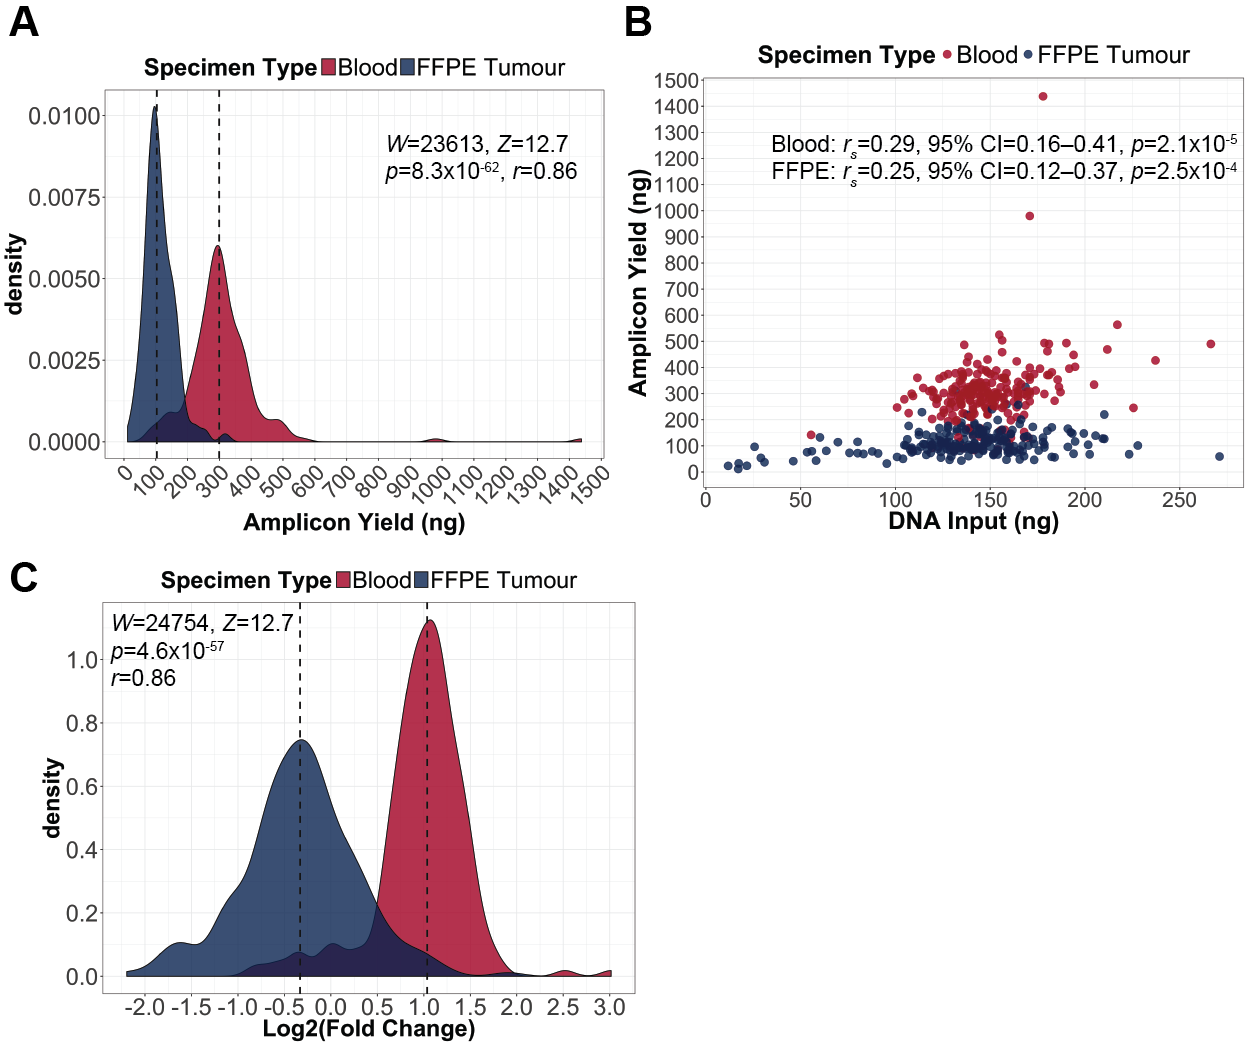
\includegraphics[scale=0.8]{dna_input_amp_yield.png}
	\caption{Comparison of efficiency in amplicon enrichment between blood and FFPE specimens. (A) Median amplicon yield is significantly lower in FFPE specimens than blood based on the Wilcoxon signed-rank test (\textit{p} $<$ 0.05). Dashed lines indicate median amplicon yield for blood and FFPE specimens. (B) Amplicon yield and DNA input for amplicon generation are weakly correlated in blood and FFPE specimens as demonstrated by Spearman's rank correlation (\textit{p} $<$ 0.05). (C) Efficiency of amplicon generation is represented by the log2 fold change between DNA input and amplicon yield (ratio of amplicon yield to DNA input). Median log2 fold change is significantly lower in FFPE specimens compared to blood as shown by the Wilcoxon signed-rank test (\textit{p} $<$ 0.05). Dashed lines indicate median log2 fold change for blood and FFPE specimens.}
	\label{fig:dna_input_amp_yield}
\end{figure}

%%%%%%%%%%%%%%%%%%%%%%%%%%%%%%%%%%%%%%%%%%%%%%%%%%%%%%%%%%%%%%%%%%%%%
%%%%%%%%%%%%%%%%%%%%%%%%%%%%%%%%%%%%%%%%%%%%%%%%%%%%%%%%%%%%%%%%%%%%%

\begin{table}[H]
\caption{Assessment of amplicon enrichment results in blood and FFPE specimens. \textit{p} value indicates significance level for Wilcoxon signed-rank test.}
\label{tbl:amplicon_generation}
			\begin{tabular}{lllllll}
				\hline
			 \multicolumn{1}{l}{ }
			 &
			 \multicolumn{2}{l}{Blood}
			 &&
			 \multicolumn{2}{l}{FFPE Tumour}
			 &
			 \multicolumn{1}{l}{ } \\
			 \cline{2-3}\cline{5-6}
			 Parameter & Median & Range && Median & Range & \textit{p} ($<$ 0.05\textsuperscript{*})
			 \\
			 \hline
			 Amplicon Yield (ng) & 299.3 & 84.0--1438.0 && 103.6 & 11.6--325.5 & \num{8.3e-62}\textsuperscript{*}
			 \\
			 DNA Input (ng) & 147.8 & 55.5--266.4 && 140.9 & 11.8--271.0 & \num{3.2e-4}\textsuperscript{*}
			 \\
			 log2(\( \frac{\text{Amplicon Yield}}{\text{DNA Input}} \)) & 1.04 & -0.845--3.01 && -0.332 & -2.20--1.90 & \num{4.6e-57}\textsuperscript{*}
			 \\
			 \hline
			\end{tabular} \\
\end{table}

%%%%%%%%%%%%%%%%%%%%%%%%%%%%%%%%%%%%%%%%%%%%%%%%%%%%%%%%%%%%%%%%%%%%%
%%%%%%%%%%%%%%%%%%%%%%%%%%%%%%%%%%%%%%%%%%%%%%%%%%%%%%%%%%%%%%%%%%%%%

\begin{figure}[H]
	\centering
	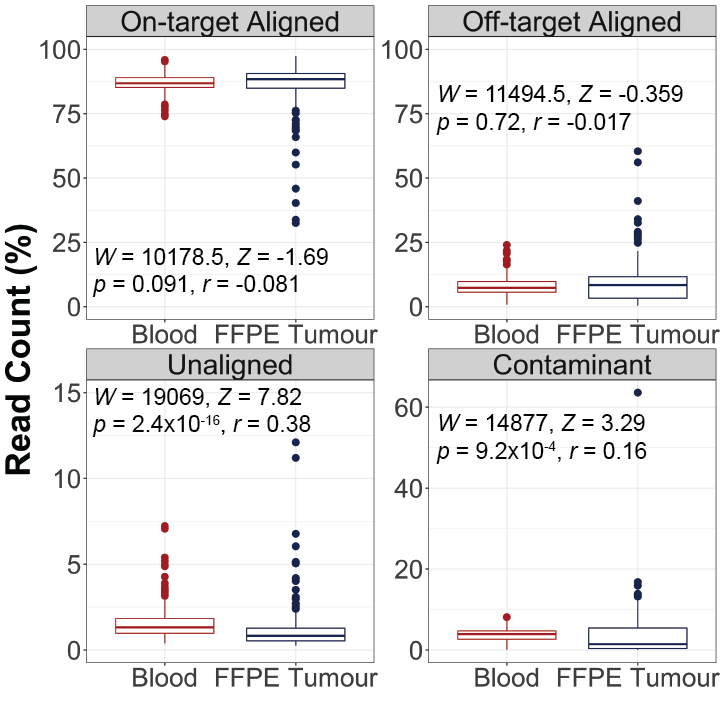
\includegraphics[scale=1]{alignment_pct.png}
	\caption{Assessment of read alignments between blood and FFPE specimens. Percentages of on-target and off-target aligned reads are not significantly different between specimen types as shown by the Wilcoxon signed-rank test, whereas percentages of unaligned and contaminant reads are significantly different (\textit{p} $<$ 0.05). Box plots show the median (horizontal bar within) and interquartile range (IQR) of percentage of reads, with whiskers representing the range of data not exceeding 1.5x the IQR and circles indicating outliers.}
	\label{fig:alignment_pct}
\end{figure}

%%%%%%%%%%%%%%%%%%%%%%%%%%%%%%%%%%%%%%%%%%%%%%%%%%%%%%%%%%%%%%%%%%%%%
%%%%%%%%%%%%%%%%%%%%%%%%%%%%%%%%%%%%%%%%%%%%%%%%%%%%%%%%%%%%%%%%%%%%%

\begin{table}[H]
\caption{Comparison of read alignments between blood and FFPE specimens. \textit{p} value indicates significance level for Wilcoxon signed-rank test.}
\label{tbl:alignment}
      \begin{tabular}{lllllll}
        \hline
				\multicolumn{1}{l}{ }
				&
				\multicolumn{2}{l}{Blood}
				&&
				\multicolumn{2}{l}{FFPE Tumour}
				&
				\multicolumn{1}{l}{ } \\
				\cline{2-3}\cline{5-6}
        Parameter & Median & Range && Median & Range & \textit{p} ($<$ 0.05\textsuperscript{*})
				\\
				\hline
				On-target Aligned Reads (\%) & 86.8 & 74.0--95.9 && 88.4 & 32.5--97.4 & \num{0.091}
				\\
				Off-target Aligned Reads (\%) & 7.3 & 0.8--24.0 && 8.4 & 0.4--60.4 & \num{0.72}
				\\
				Unaligned Reads (\%) & 1.3 & 0.4--7.2 && 0.8 & 0.3--12.1 & \num{2.4e-16}\textsuperscript{*}
				\\
				Contaminant (\%) & 3.9 & 0.1--8.1 && 1.4 & 0.03--63.6 &
				\num{9.2e-4}\textsuperscript{*}
				\\
				\hline
      \end{tabular} \\
\end{table}

%%%%%%%%%%%%%%%%%%%%%%%%%%%%%%%%%%%%%%%%%%%%%%%%%%%%%%%%%%%%%%%%%%%%%
%%%%%%%%%%%%%%%%%%%%%%%%%%%%%%%%%%%%%%%%%%%%%%%%%%%%%%%%%%%%%%%%%%%%%

\begin{figure}[H]
	\centering
	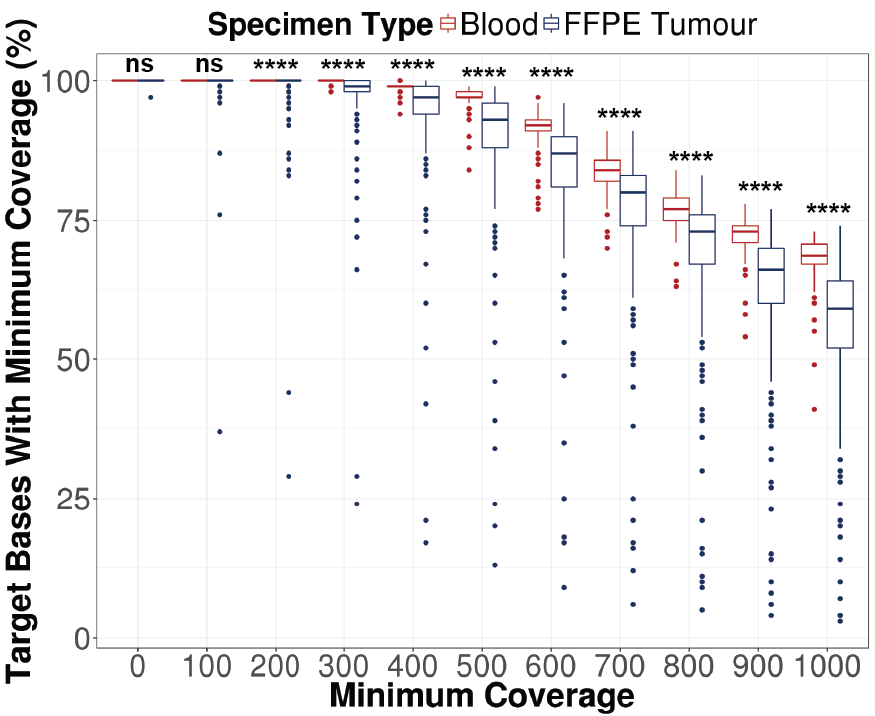
\includegraphics[scale=0.9]{coverage_stats.png}
	\caption{Evaluation of coverage uniformity in blood and FFPE specimens. Per base coverage was normalized to account for difference in library size. Percentage of target bases that met various coverage thresholds was calculated. Wilcoxon signed-rank test showed significant differences in percentage of target bases at all coverage thresholds except at the zero coverage cut-off (****\textit{p} $<$ 0.0001, ***\textit{p} $<$ 0.001, **\textit{p} $<$ 0.01, *\textit{p} $<$ 0.05, ns = not significant). Box plots show the median (horizontal bar within) and interquartile range (IQR) of percentage of target bases that meet the respective coverage thresholds, with whiskers representing the range of data not exceeding 1.5x the IQR and circles indicating outliers.}
	\label{fig:coverage_stats}
\end{figure}

%%%%%%%%%%%%%%%%%%%%%%%%%%%%%%%%%%%%%%%%%%%%%%%%%%%%%%%%%%%%%%%%%%%%%
%%%%%%%%%%%%%%%%%%%%%%%%%%%%%%%%%%%%%%%%%%%%%%%%%%%%%%%%%%%%%%%%%%%%%

\begin{table}[H]
\caption{Assessment of coverage uniformity between blood and FFPE specimens using the Wilcoxon signed-rank test.}
\label{tbl:metrics}
\centering
      \begin{tabular}{llllllllll}
        \hline
				\multicolumn{1}{l}{ }
				&
				\multicolumn{2}{l}{Blood}
				&&
				\multicolumn{2}{l}{FFPE Tumour}
				&
				\multicolumn{4}{l}{ } \\
				\cline{2-3}\cline{5-6}
        Threshold & Median (\%) & Range (\%) && Median (\%) & Range (\%) & \textit{W} & \textit{Z} & \textit{p} ($<$ 0.05\textsuperscript{*}) & \textit{r}
				\\
				\hline
				$\geq$ 0x & 100.0 & 100.0--100.0 && 100.0 & 97.0--100.0 & 1 & 1.00 & 1.0 & 0.068
				\\
				$\geq$ 100x & 100.0 & 100.0--100.0 && 100.0 & 37.0--100.0 & 91 & 3.61 & \num{2.3e-4}\textsuperscript{*} & 0.25
				\\
				$\geq$ 200x & 100.0 & 100.0--100.0 && 100.0 & 29.0--100.0 & 666 & 5.99 & \num{2.9e-11}\textsuperscript{*} & 0.41
				\\
				$\geq$ 300x & 100.0 & 98.0--100.0 && 99.0 & 24.0--100.0 & 7696 & 8.17 & \num{4.1e-18}\textsuperscript{*} & 0.55
				\\
				$\geq$ 400x & 99.0 & 94.0--100.0 && 97.0 & 17.0--100.0 & 13934 & 10.0 & \num{5.0e-28}\textsuperscript{*} & 0.68
				\\
				$\geq$ 500x & 97.0 & 84.0--99.0 && 89.5 & 13.0--99.0 & 19880.5 & 11.3 & \num{2.1e-38}\textsuperscript{*} & 0.77
				\\
				$\geq$ 600x & 92.0 & 77.0--97.0 && 87.0 & 9.0--96.0 & 20762 & 10.6 & \num{1.5e-32}\textsuperscript{*} & 0.72
				\\
				$\geq$ 700x & 84.0 & 70.0--91.0 && 80.0 & 6.0--91.0 & 18458.5 & 9.54 & \num{5.7e-25}\textsuperscript{*} & 0.65
				\\
				$\geq$ 800x & 77.0 & 63.0-84.0 && 73.0 & 5.0--83.0 & 18127 & 9.87 & \num{4.7e-27}\textsuperscript{*} & 0.67
				\\
				$\geq$ 900x & 73.0 & 54.0--78.0 && 66.0 & 4.0--77.0 & 20706 & 11.5 & \num{4.6e-40}\textsuperscript{*} & 0.78
				\\
				$\geq$ 1000x & 68.5 & 41.0--73.0 && 59.0 & 3.0-74.0 & 21054.5 & 11.7 & \num{3.6e-42}\textsuperscript{*} & 0.79
				\\
				\hline
      \end{tabular} \\
\end{table}

%%%%%%%%%%%%%%%%%%%%%%%%%%%%%%%%%%%%%%%%%%%%%%%%%%%%%%%%%%%%%%%%%%%%%
\section{Reduced coverage depth in FFPE specimens is more pronounced for longer amplicons}
\label{sec:ReducedcoveragedepthinFFPEspecimensismorepronouncedforlongeramplicons}

The OncoPanel consists of 416 amplicons that interrogate coding exons and clinically relevant hotpots of 21 genes, and these amplicons vary in length and GC content. Since we observed discrepancy in sequencing coverage between blood and FFPE specimens, we sought to determine whether this discrepancy is influenced by amplicon length and GC content. We attained the coverage depth for each amplicon and normalized the coverage depth to account for difference in library size. We found significant difference in coverage depth between blood and FFPE specimens for 331 out of 416 amplicons (Wilcoxon signed-rank test with Benjamini-Hochberg correction, adjusted \textit{p} $<$ 0.0001; \autoref{fig:amp_norm_depth_med_wilcoxon_volcano}). To quantify the discrepancy in amplicon coverage depth between specimen types, we derived the log2 fold change from the median coverage depth in blood specimens to the median coverage depth in FFPE specimens (log2\( \frac{\text{Median Coverage Depth in FFPE}}{\text{Median Coverage Depth in Blood}} \)) for each amplicon. Hence, a negative fold change indicates lower coverage depth of the amplicon in FFPE specimens relative to blood specimens, whereas a positive fold change indicates higher coverage depth of the amplicon in FFPE specimens relative to blood specimens. Our assessment showed that 217 out of the 331 amplicons have negative log2 fold changes, whereas 114 out of the 331 amplicons have positive log2 fold changes (\autoref{fig:amp_norm_depth_med_wilcoxon_volcano}). These results indicate that there are differences in coverage depth between FFPE and blood specimens for the majority of amplicons in the panel, with more amplicons exhibiting lower coverage depth in FFPE specimens than blood specimens.

We subsequently examined the impact of amplicon length and GC content on the discrepancy in amplicon coverage depth between FFPE and blood specimens. We first confirmed that no significant correlation exists between amplicon GC content and length (Pearson's correlation, \textit{r} = 0.045, 95\% CI = -0.051--0.14, \textit{p} = 0.36). We then explored the correlation between the median coverage depth of amplicons and amplicon length in both blood and FFPE specimens (\autoref{fig:amp_cov_lm_len}A). While we found no significant correlation between median coverage depth and amplicon length in blood specimens (Pearson's correlation, \textit{r} = 0.042, 95\% CI = -0.054--0.14, \textit{p} = 0.39), we observed a negative correlation in FFPE specimens (Pearson's correlation, \textit{r} = -0.28, 95\% CI = -0.37-- -0.19, \textit{p} = \num{7.4e-9}). We evaluated the relationship between the discrepancy in amplicon coverage depth between FFPE and blood specimens, which was calculated as the log2 fold change from the median coverage depth in blood specimens to the median coverage depth in FFPE specimens (log2\( \frac{\text{Median Coverage Depth in FFPE}}{\text{Median Coverage Depth in Blood}} \)), and amplicon length (\autoref{fig:amp_cov_lm_len}B). Pearson's correlation demonstrated a strong, negative correlation between the log2 fold change in amplicon coverage depth and amplicon length (\textit{r} = \mbox{-0.79}, 95\% CI = -0.82-- -0.75, \textit{p} = \num{1.4e-88}), indicating that the decline in amplicon coverage depth in FFPE specimens relative to blood specimens becomes larger as amplicon length increases.

To assess the effect of amplicon GC content on coverage depth of amplicons, we explored the correlation between the median coverage depth of amplicons and amplicon GC content in blood and FFPE specimens (\autoref{fig:amp_cov_lm_gc}A). Using Pearson's correlation, we identified weak, negative correlations between median coverage depth and amplicon GC content in both blood and FFPE specimens (blood: \textit{r} = -0.16, 95\% CI = -0.25-- -0.067, \textit{p} = \num{8.7e-4}; FFPE: \textit{r} = -0.29, 95\% CI = -0.38-- -0.20 \textit{p} = \num{1.0e-9}). We next assessed the relationship between the discrepancy in amplicon coverage depth between FFPE and blood specimens (log2\( \frac{\text{Median Coverage Depth in FFPE}}{\text{Median Coverage Depth in Blood}} \)) and amplicon GC content (\autoref{fig:amp_cov_lm_gc}B). In contrast to the strong, negative correlation observed for the log2 fold change in amplicon coverage depth in relation to amplicon length, Pearson's correlation demonstrated a weak, negative correlation between the log2 fold change in amplicon coverage depth and amplicon GC content (\textit{r} = -0.31, 95\% CI = -0.40-- -0.22, \textit{p} = \num{1.1e-10}). While the correlation is weak, this finding still implies that increased amplicon GC content has a significant impact on the decrease in amplicon coverage depth in FFPE specimens relative to blood specimens.

Because amplicon length and GC content demonstrated significant effects on the discrepancy in amplicon coverage depth between FFPE and blood specimens, we sought to determine which contributing factor has a greater effect. We used a multiple linear regression to predict log2 fold change in amplicon coverage depth between blood and FFPE specimens (log2\( \frac{\text{Median Coverage Depth in FFPE}}{\text{Median Coverage Depth in Blood}} \)) based on amplicon length and GC content (\autoref{tbl:multiple_regression}). A significant equation was found (\textit{F}(2, 411) = 471, \textit{p} = \num{4.65e-107}), with an adjusted \textit{R\textsuperscript{2}} of 0.695. Predicted fold change in amplicon coverage depth between blood and FFPE specimens (log2) is equal to 1.66-\num{7.24e-3}(\textit{Amplicon Length})-\num{9.92e-3}(\textit{Amplicon GC Content}), in which amplicon length is expressed in base pairs (bp) and GC content is expressed as percentage (\%). Both amplicon length and GC content were significant predictors of log2 fold change in amplicon coverage depth between blood and FFPE specimens. Based on the standardized coefficients, we compared the strength of predictors within the model to identify the predictor with a greater effect on the response variable. Our assessment showed that one standard deviation increase in amplicon length would lead to a -0.775 standard deviation decrease in log2 fold change in amplicon coverage depth between blood and FFPE specimens, whereas one standard deviation increase in amplicon GC content would lead to a -0.277 standard deviation decrease in the response variable. This result indicates that amplicon length has a stronger association with the fold change in amplicon coverage depth between blood and FFPE specimens (log2) than amplicon GC content. Together, these findings reflect the challenges imposed by fragmentation damages in FFPE DNA: formalin fixation induces DNA fragmentation, resulting in shorter template DNA that would be more difficult for PCR amplification to generate longer amplicons.

%%%%%%%%%%%%%%%%%%%%%%%%%%%%%%%%%%%%%%%%%%%%%%%%%%%%%%%%%%%%%%%%%%%%%
%%%%%%%%%%%%%%%%%%%%%%%%%%%%%%%%%%%%%%%%%%%%%%%%%%%%%%%%%%%%%%%%%%%%%

\begin{figure}[H]
	\centering
	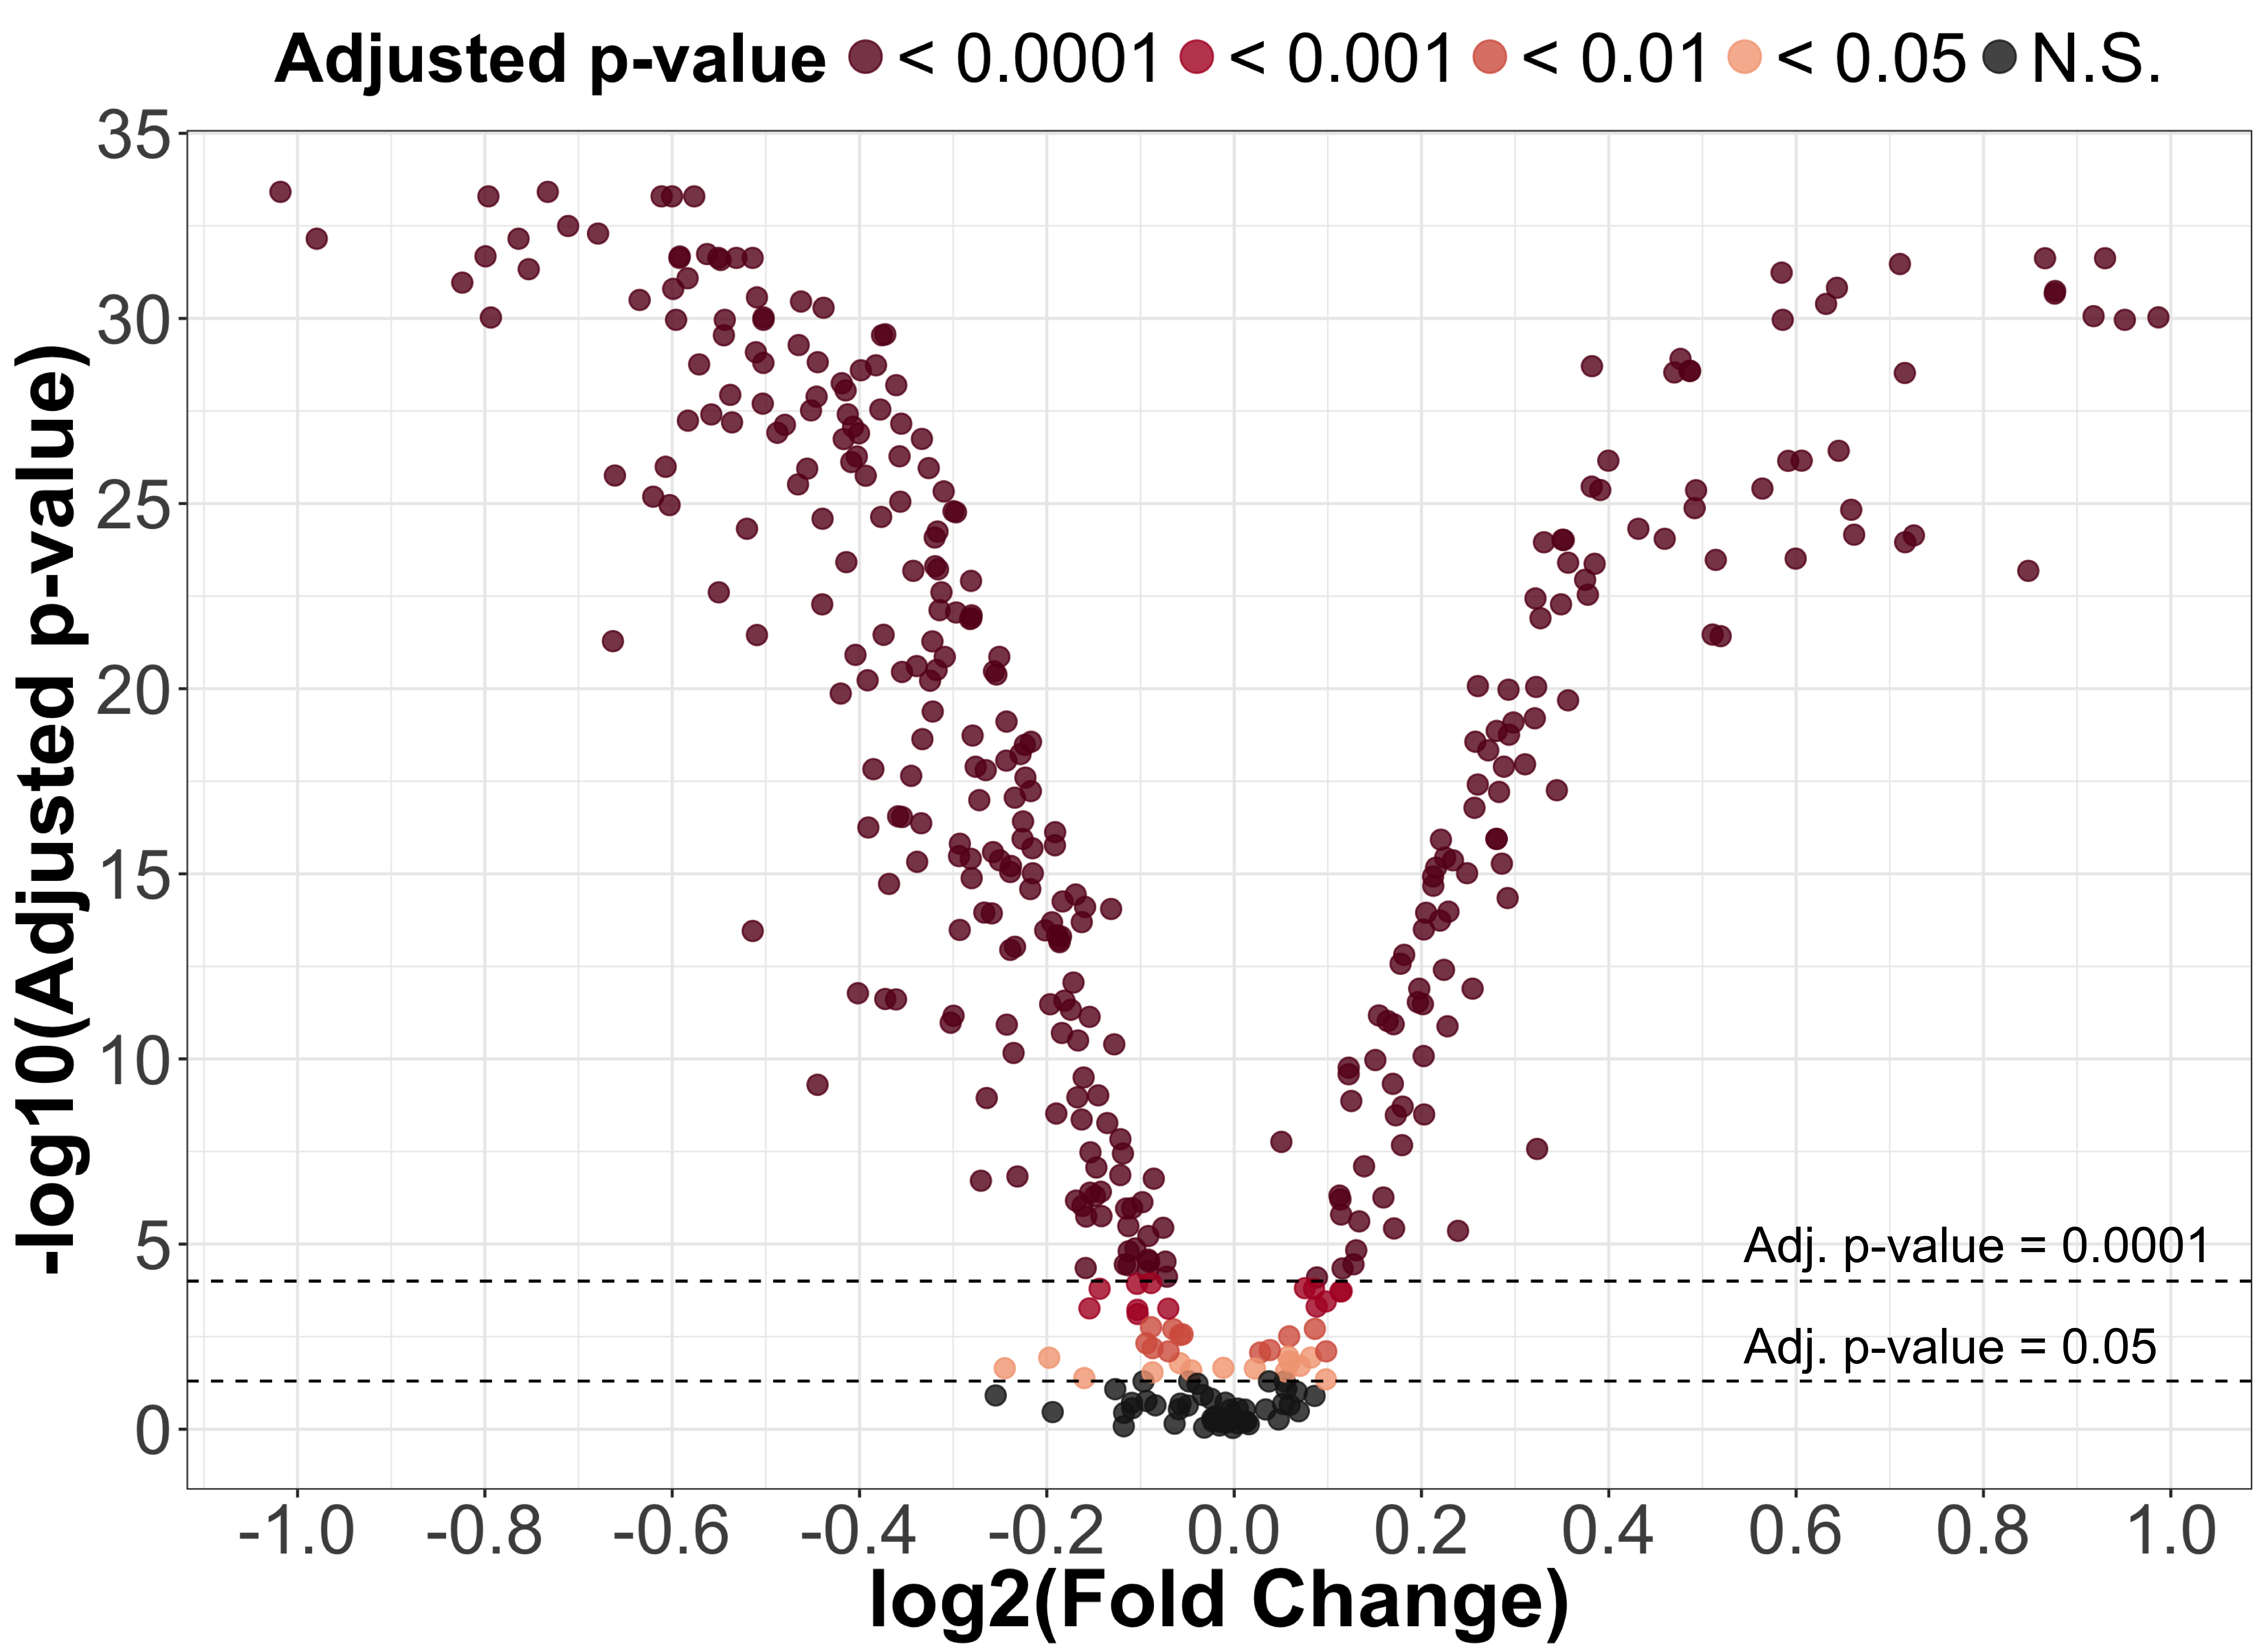
\includegraphics[scale=0.14]{amp_norm_depth_med_wilcoxon_volcano.png}
	\caption{Coverage depth is significantly different between FFPE and blood specimens for the majority of amplicons in the OncoPanel (Wilcoxon signed-rank test with Benjamini-Hochberg correction, adjusted \textit{p} $<$ 0.0001). Amplicon coverage depth was normalized to account for difference in library size and log2 fold change between the median coverage depth in blood and FFPE specimens (log2\( \frac{\text{Median Coverage Depth in FFPE}}{\text{Median Coverage Depth in Blood}} \)) was calculated for each amplicon. Volcano plot illustrates -log10 adjusted \textit{p}-value in relation to log2 fold change. Negative log2 fold change indicates lower amplicon coverage depth in FFPE specimens than blood specimens ($\downarrow \text{Coverage\textsubscript{FFPE}}$), whereas positive log2 fold change indicates higher amplicon coverage depth in FFPE specimens than blood specimens ($\uparrow\text{Coverage\textsubscript{FFPE}}$). N = number of amplicons.}
	\label{fig:amp_norm_depth_med_wilcoxon_volcano}
\end{figure}

%%%%%%%%%%%%%%%%%%%%%%%%%%%%%%%%%%%%%%%%%%%%%%%%%%%%%%%%%%%%%%%%%%%%%
%%%%%%%%%%%%%%%%%%%%%%%%%%%%%%%%%%%%%%%%%%%%%%%%%%%%%%%%%%%%%%%%%%%%%

\begin{figure}[H]
	\centering
	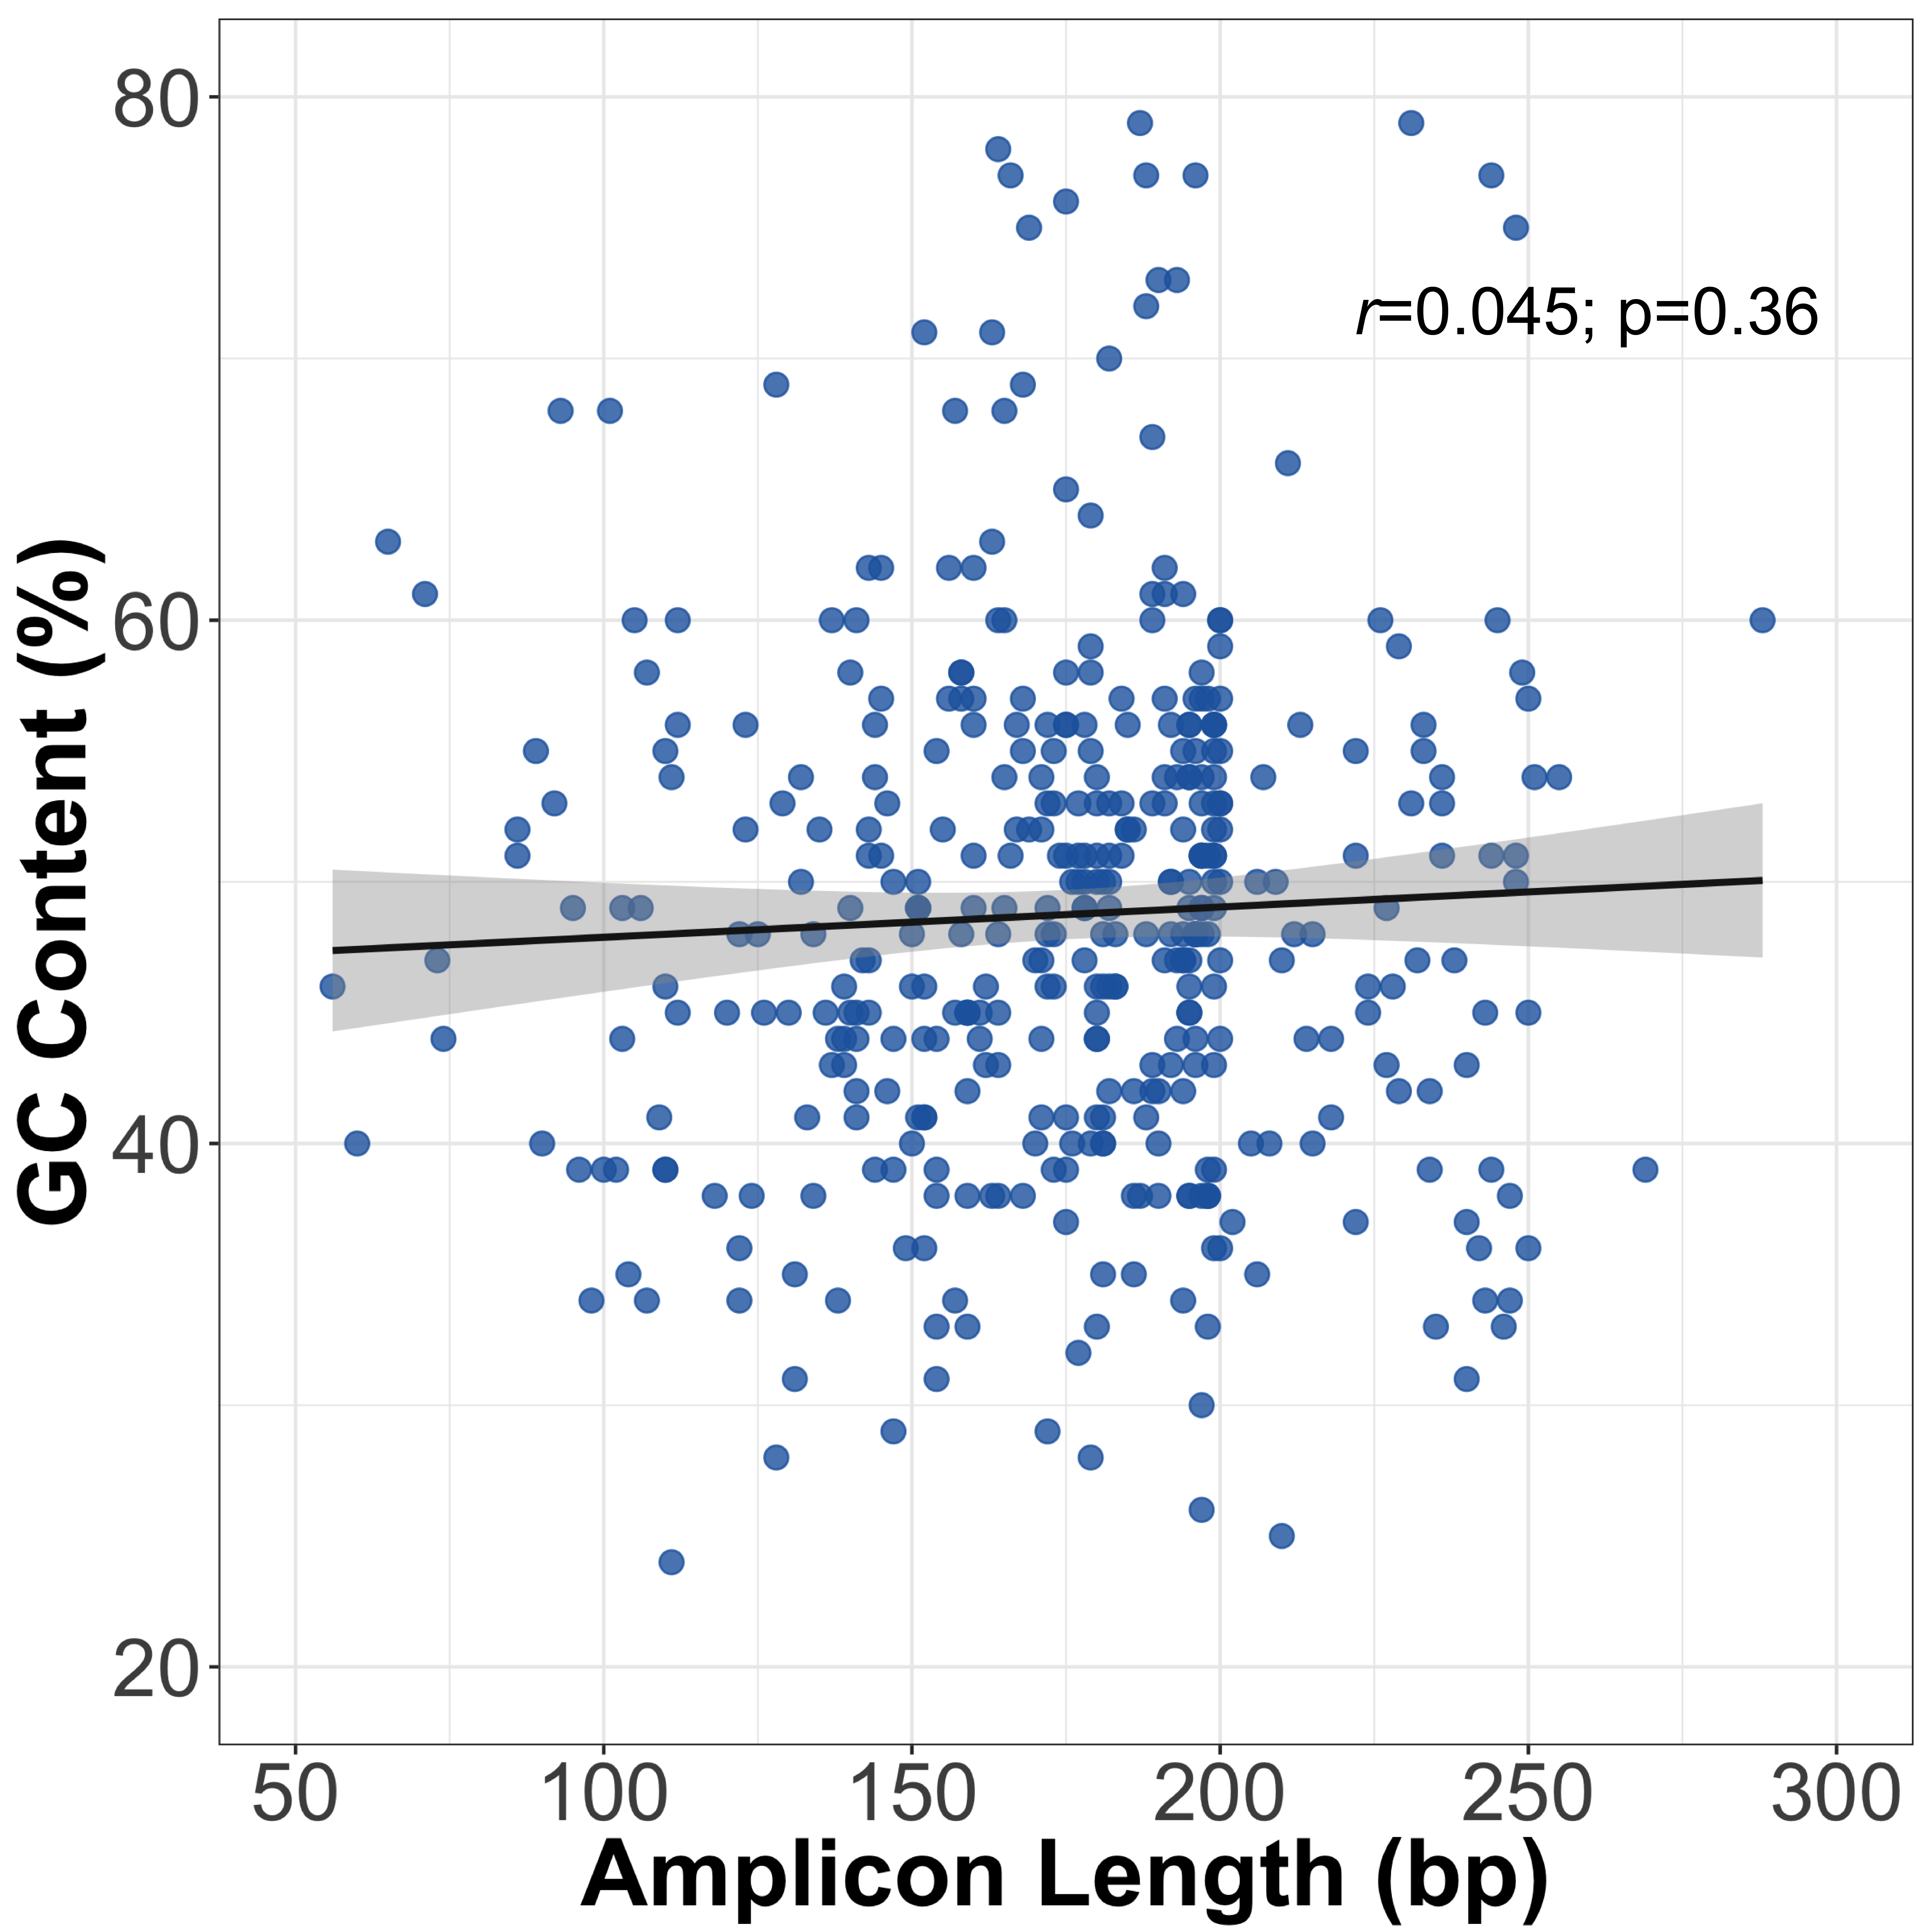
\includegraphics[scale=0.14]{amp_gc_length.png}
	\caption{The relationship between amplicon GC content (\%) and amplicon length (bp). Pearson's correlation showed that amplicon GC content is not significantly correlated with amplicon length (\textit{p} $<$ 0.05).}
	\label{fig:amp_gc_length}
\end{figure}

%%%%%%%%%%%%%%%%%%%%%%%%%%%%%%%%%%%%%%%%%%%%%%%%%%%%%%%%%%%%%%%%%%%%%
%%%%%%%%%%%%%%%%%%%%%%%%%%%%%%%%%%%%%%%%%%%%%%%%%%%%%%%%%%%%%%%%%%%%%

\begin{figure}[H]
	\centering
	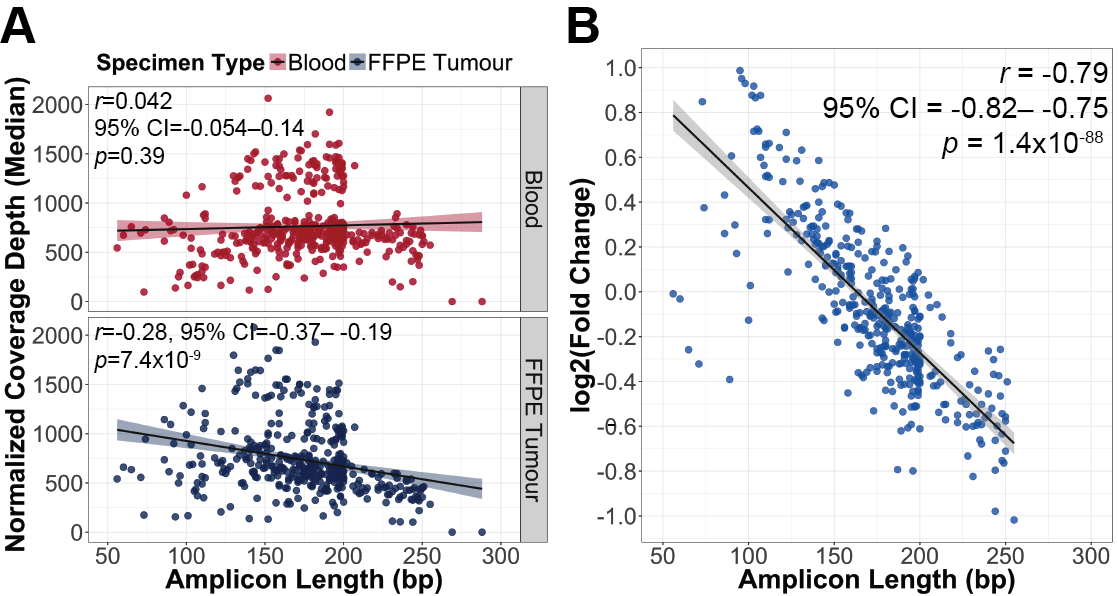
\includegraphics[scale=0.85]{amp_cov_lm_len.png}
	\caption{The effect of amplicon length on coverage depth of amplicons. Coverage depth of amplicons was normalized to account for difference in library size and log2 fold change between the median coverage depth in blood and FFPE specimens (log2\( \frac{\text{Median Coverage Depth in FFPE}}{\text{Median Coverage Depth in Blood}} \)) was calculated for each amplicon. (A) No significant correlation between coverage depth of amplicons and amplicon length was demonstrated in blood specimens, whereas coverage depth of amplicons is negatively correlated with amplicon length in FFPE specimens (Pearson's correlation, \textit{p} $<$ 0.05). (B) Increased in amplicon length leads to lower log2 fold change in amplicon coverage depth between blood and FFPE specimens (Pearson's correlation, \textit{p} $<$ 0.05).}
	\label{fig:amp_cov_lm_len}
\end{figure}

%%%%%%%%%%%%%%%%%%%%%%%%%%%%%%%%%%%%%%%%%%%%%%%%%%%%%%%%%%%%%%%%%%%%%
%%%%%%%%%%%%%%%%%%%%%%%%%%%%%%%%%%%%%%%%%%%%%%%%%%%%%%%%%%%%%%%%%%%%%

\begin{figure}[H]
	\centering
	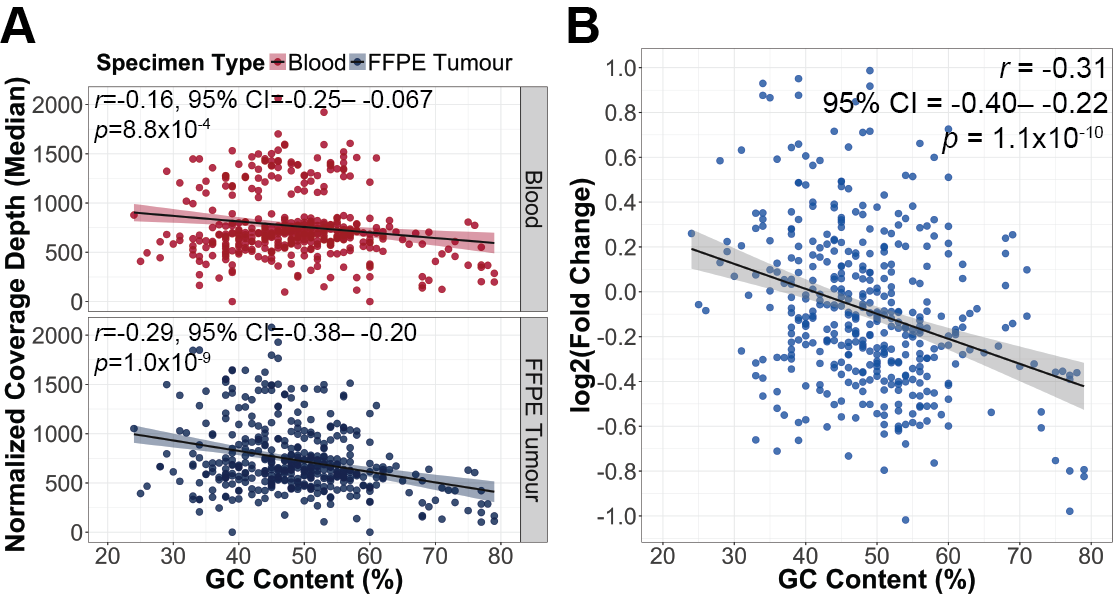
\includegraphics[scale=0.85]{amp_cov_lm_gc.png}
	\caption{The effect of amplicon GC content on coverage depth of amplicons. Coverage depth of amplicons was normalized to account for difference in library size and log2 fold change between the median coverage depth in blood and FFPE specimens (log2\( \frac{\text{Median Coverage Depth in FFPE}}{\text{Median Coverage Depth in Blood}} \)) was calculated for each amplicon. (A) Coverage depth of amplicons is negatively correlated with amplicon GC content in both blood and FFPE specimens (Pearson's correlation, \textit{p} $<$ 0.05). (B) Increased in amplicon GC content leads to lower log2 fold change in amplicon coverage depth between blood and FFPE specimens (Pearson's correlation, \textit{p} $<$ 0.05).}
	\label{fig:amp_cov_lm_gc}
\end{figure}

%%%%%%%%%%%%%%%%%%%%%%%%%%%%%%%%%%%%%%%%%%%%%%%%%%%%%%%%%%%%%%%%%%%%%
%%%%%%%%%%%%%%%%%%%%%%%%%%%%%%%%%%%%%%%%%%%%%%%%%%%%%%%%%%%%%%%%%%%%%

\begin{table}[H]
\caption{Multiple linear regression to predict log2 fold change in amplicon coverage depth between blood and FFPE specimens based on amplicon length and GC content.}
\label{tbl:multiple_regression}
\centering
      \begin{tabular}{l|ccccl}
        Variable & Unstandardized Coefficient & Standard Error & Standardized Coefficient & \textit{p}-value
        \\
        \hline
        Length (bp) & \num{-7.24e-3} & \num{2.54e-4} & \num{-7.75e-1} & \num{2.47e-99}
				\\
				GC Content (\%) & \num{-9.92e-3} & \num{9.77e-4} & \num{-2.77e-1} & \num{8.70e-22}
				\\
				\hline
				\\
				 & \multicolumn{4}{r}{Intercept = 1.66, Adjusted R\textsuperscript{2} = 0.695}
				\\
				 & \multicolumn{4}{r}{\textit{F}(2, 411) = 471, \textit{p}-value = \num{4.65e-107}}
				\\
				\hline
      \end{tabular} \\
\end{table}

%%%%%%%%%%%%%%%%%%%%%%%%%%%%%%%%%%%%%%%%%%%%%%%%%%%%%%%%%%%%%%%%%%%%%
\section{Deamination effects lead to increased C$>$T/G$>$A transitions in FFPE specimens}
\label{sec:DeaminationeffectsleadtoincreasedC$>$T/G$>$AtransitionsatlowallelefrequencyinFFPEspecimens}

Formalin fixation not only induces DNA fragmentation, but also causes deamination of cytosine bases, leading to increase in C$>$T/G$>$A transitions. To measure the level of formalin-induced artifacts in FFPE specimens, we quantified the fraction of base changes that were not identified as true SNVs by our variant calling pipeline. We only considered high quality bases (Phred-scaled base quality score $\geq$ 20) and base changes that were $\geq$ 1\% allele frequency to avoid inclusion of sequencing errors in our analysis. Base changes were categorized into C$>$T/G$>$A, A$>$G/T$>$C, C$>$A/G$>$T, A$>$C/T$>$G, C$>$G/G$>$C, and A$>$T/T$>$A, and we compared the fraction of base changes between blood and FFPE specimens.

Formalin fixation not only induces DNA fragmentation, but also causes deamination of cytosine bases, leading to increase in C$>$T/G$>$A transitions. To measure the level of formalin-induced artifacts in FFPE specimens, we quantified the fraction of base changes that were not identified as true SNVs by our variant calling pipeline. We only considered high quality bases (Phred-scaled base quality score $\geq$ 20) and base changes that were $\geq$ 1\% allele frequency to avoid inclusion of sequencing errors in our analysis. We found significant difference in fraction of base changes

%%%%%%%%%%%%%%%%%%%%%%%%%%%%%%%%%%%%%%%%%%%%%%%%%%%%%%%%%%%%%%%%%%%%%
%%%%%%%%%%%%%%%%%%%%%%%%%%%%%%%%%%%%%%%%%%%%%%%%%%%%%%%%%%%%%%%%%%%%%

\begin{figure}[H]
	\centering
	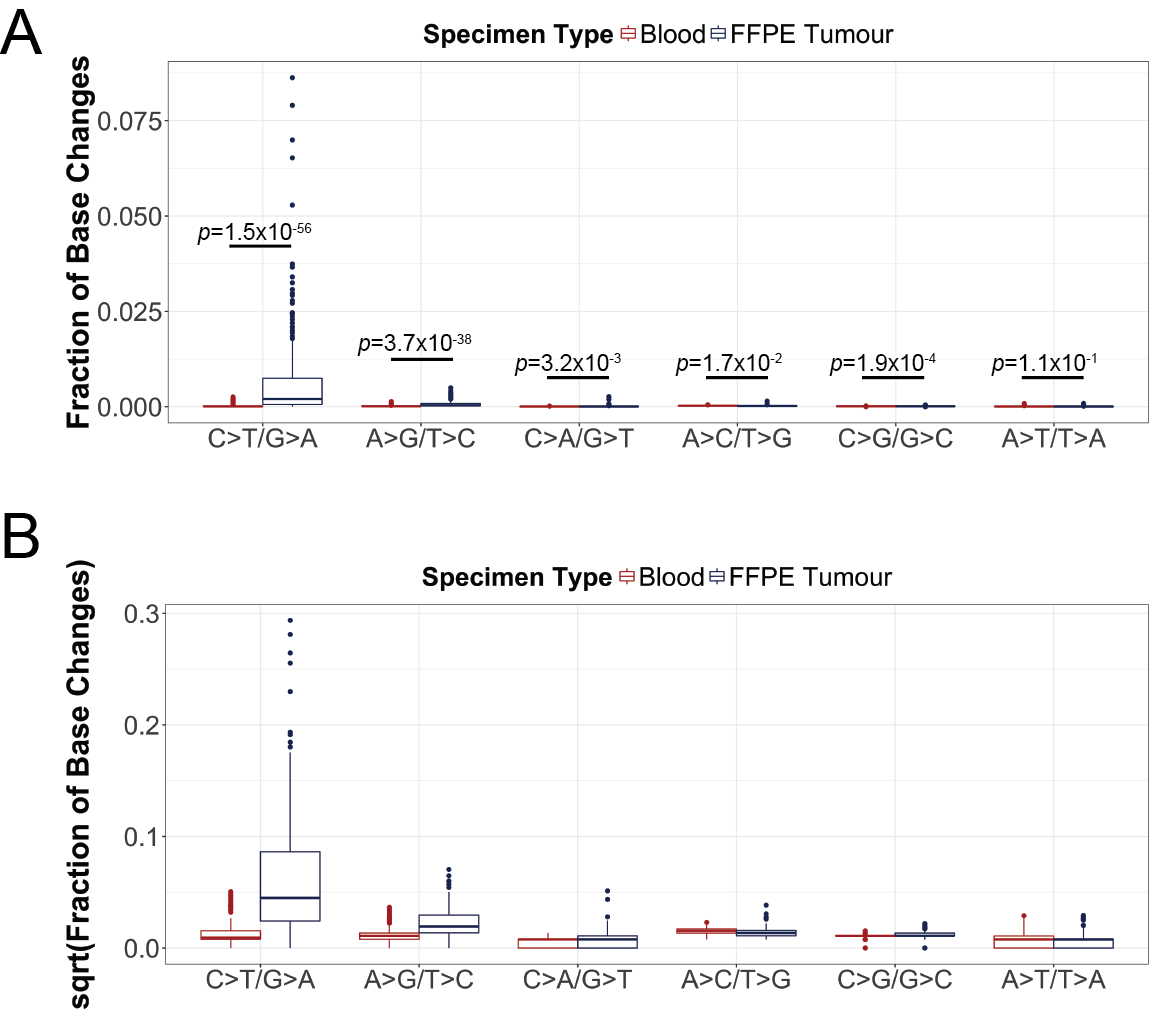
\includegraphics[scale=0.8]{deamination_effect_blood_ffpe.png}
	\caption{Detection of formalin-induced sequence artifacts in FFPE specimens. (A) }
	\label{fig:deamination_effect_blood_ffpe}
\end{figure}

%%%%%%%%%%%%%%%%%%%%%%%%%%%%%%%%%%%%%%%%%%%%%%%%%%%%%%%%%%%%%%%%%%%%%
%%%%%%%%%%%%%%%%%%%%%%%%%%%%%%%%%%%%%%%%%%%%%%%%%%%%%%%%%%%%%%%%%%%%%

\begin{table}[H]
\caption{Multiple pairwise comparison of log2 fold change in fraction of base changes between FFPE and blood specimens using Dunn's test with Benjamini-Hochberg multiple hypothesis testing correction. Top values represent Dunn's pairwise \textit{z} statistics, whereas bottom values represent adjusted \textit{p}-value. Asterisk(*) indicates significance level of adjusted \textit{p}-value $<$ 0.05.}
\label{dunntest}
\centering
      \begin{tabular}{r|l|l|l|l|ll}
        Type of Base Changes & A$>$C/T$>$G & A$>$G/T$>$C & A$>$T/T$>$A & C$>$A/G$>$T & C$>$G/G$>$C
        \\
        \hline
        A$>$G/T$>$C & -11.7 &  &  &  &
        \\
				 & \num{4.15e-31}\mbox{*} &  &  &  &
				\\
				\hline
        A$>$T/T$>$A & -0.399 & 9.57 &  &  &
        \\
				 & \num{3.45e-1} & \num{1.31e-21}\mbox{*} & & &
				\\
				\hline
        C$>$A/G$>$T & -3.46 & 6.39 & -2.73 &  &
        \\
				 & \num{4.00e-4}\mbox{*} & \num{1.52e-10}\mbox{*} & \num{3.99e-3}\mbox{*} & &
				\\
				\hline
        C$>$G/G$>$C & -3.02 & 8.63 & -2.17 & 0.918 &
				\\
				 & \num{1.73e-3}\mbox{*} & \num{6.76e-18}\mbox{*} & \num{1.71e-2}\mbox{*} & \num{1.92e-1} &
        \\
				\hline
        C$>$T/G$>$A & -17.1 & -5.60 & -14.3 & -11.1 & -14.1
        \\
				 & \num{7.78e-65}\mbox{*} & \num{1.76e-8}\mbox{*} & \num{5.10e-46}\mbox{*} & \num{1.32e-28}\mbox{*} & \num{6.46e-45}\mbox{*}
				 \\
				\hline
      \end{tabular} \\
\end{table}

%%%%%%%%%%%%%%%%%%%%%%%%%%%%%%%%%%%%%%%%%%%%%%%%%%%%%%%%%%%%%%%%%%%%%
%%%%%%%%%%%%%%%%%%%%%%%%%%%%%%%%%%%%%%%%%%%%%%%%%%%%%%%%%%%%%%%%%%%%%

\begin{figure}[H]
	\centering
	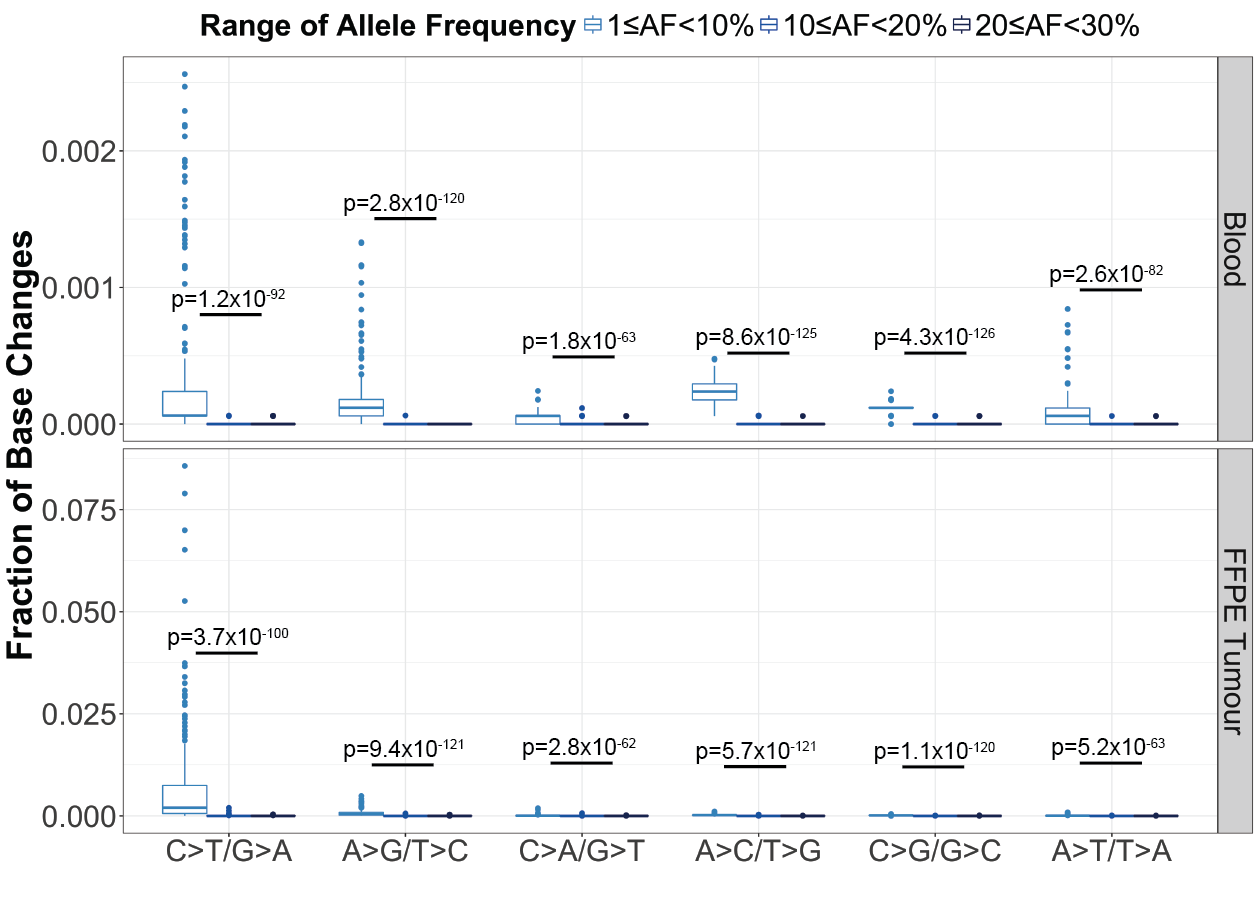
\includegraphics[scale=0.8]{deamination_effect_af_range.png}
	\caption{Add caption.}
	\label{fig:deamination_effect_af_range}
\end{figure}

%%%%%%%%%%%%%%%%%%%%%%%%%%%%%%%%%%%%%%%%%%%%%%%%%%%%%%%%%%%%%%%%%%%%%
%%%%%%%%%%%%%%%%%%%%%%%%%%%%%%%%%%%%%%%%%%%%%%%%%%%%%%%%%%%%%%%%%%%%%


%%%%%%%%%%%%%%%%%%%%%%%%%%%%%%%%%%%%%%%%%%%%%%%%%%%%%%%%%%%%%%%%%%%%%
\section{Increased age of paraffin block results in reduced amplicon yield and elevated events of C$>$T/G$>$A sequence artifacts}
\label{sec:IncreasedageofparaffinblockresultsinpoorerampliconyieldandelevatedeventsofC$>$T/G$>$Asequenceartifacts}

The amount of amplifiable DNA derived from FFPE specimens is dependent on the extent of fragmentation damages. Given two DNA samples of similar quantity, the sample with more extensive DNA fragmentation would yield reduced amount of PCR amplicons compared to the less fragmented sample.

\begin{figure}[H]
	\centering
	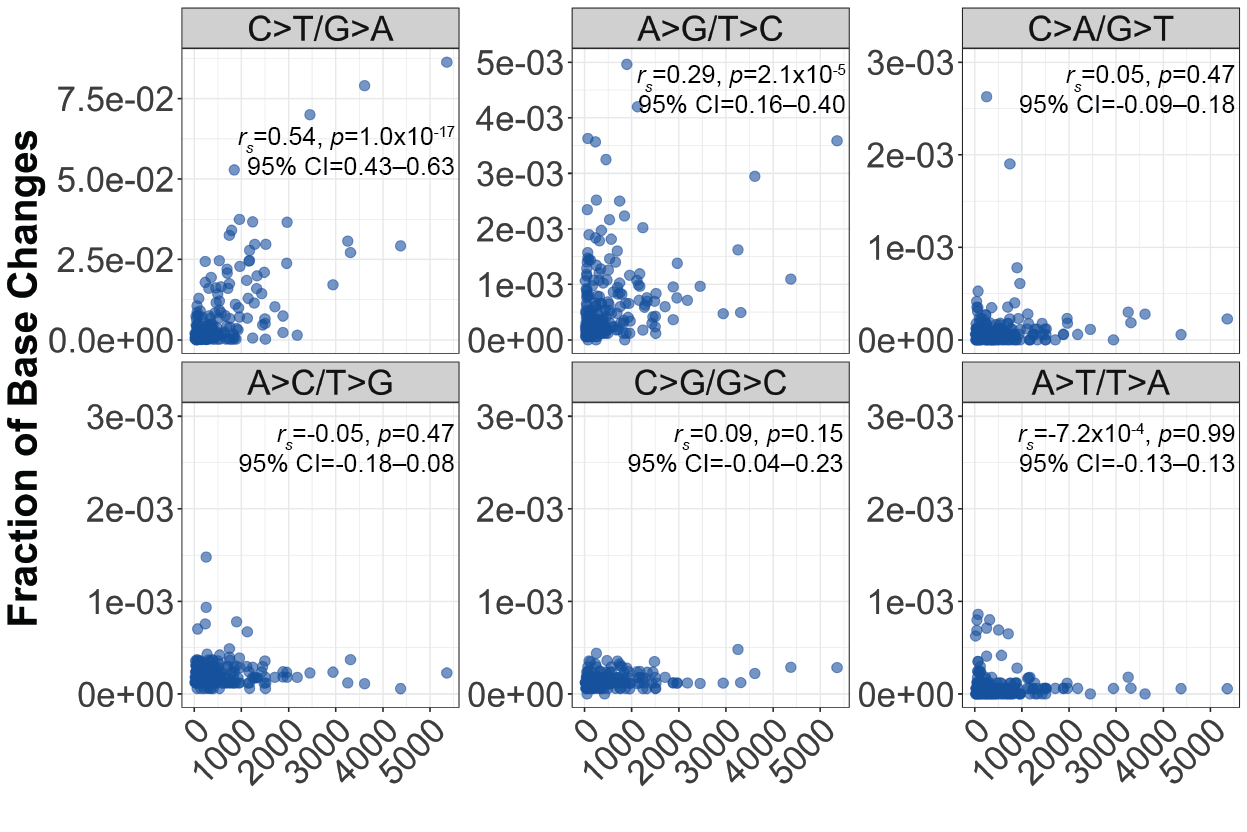
\includegraphics[scale=0.8]{deamination_effect_age.png}
	\caption{Add caption.}
	\label{fig:deamination_effect_age}
\end{figure}

\begin{table}[H]
\caption{Determination of correlation between pre-sequencing variables and sequencing results using Spearman's correlation. Top values represent Spearman's \textit{rho} and 95\% confidence interval in brackets, whereas bottom values represent \textit{p}-value. Asterisk(*) indicates significance level of \textit{p}-value $<$ 0.05.}
\label{spearman_corr}
\centering
      \begin{tabular}{l|l|l|l|ll}
        Variable & Amplicon & Age of Paraffin & Fraction of & Average Per Base
        \\
				 & Yield (ng) & Block (Day) & C$>$T/G$>$A & Normalized Coverage
				\\
        \hline
        Age of Paraffin & -0.42 (-0.52-- -0.30) & & &
				\\
				Block (Day) & \num{5.2e-7}\mbox{*} & & &
        \\
				\hline
				Fraction of & -0.72 (-0.77-- -0.65) & 0.54 (0.61--0.75) & &
				\\
				C$>$T/G$>$A & \num{1.9e-11}\mbox{*} & \num{6.3e-35}\mbox{*} & &
				\\
				\hline
				Average Per Base & 0.69 (0.61--0.75) & -0.47 (-0.57-- -0.36) & -0.80 (-0.84-- -0.75) &
				\\
				Normalized Coverage & \num{8.5e-20}\mbox{*} & \num{4.7e-7}\mbox{*} & \num{7.5e-17}\mbox{*} &
				\\
				\hline
				On-target & 0.58 (0.48--0.66) & -0.35 (-0.46-- -0.23) & -0.57 (-0.65-- -0.47) & 0.73 (0.66--0.79)
				\\
				Aligned Reads (\%) & \num{2.1e-13}\mbox{*} & \num{8.2e-3}\mbox{*} & \num{4.2e-8}\mbox{*} & \num{3.1e-58}\mbox{*}
				\\
				\hline
      \end{tabular} \\
\end{table}

%%%%%%%%%%%%%%%%%%%%%%%%%%%%%%%%%%%%%%%%%%%%%%%%%%%%%%%%%%%%%%%%%%%%%
\section{Non-reproducible variant calls are detected in sequencing replicates of FFPE specimens}
\label{sec:}

%%%%%%%%%%%%%%%%%%%%%%%%%%%%%%%%%%%%%%%%%%%%%%%%%%%%%%%%%%%%%%%%%%%%%
\section{Discussion}
\label{sec:Discussion}
%%%%%%%%%%%%%%%%%%%%%%%%%%%%%%%%%%%%%%%%%%%%%%%%%%%%%%%%%%%%%%%%%%%%%
